\documentclass[11pt]{article}
\usepackage{graphicx}
%
% This is from the HimL deliverable
%

\begin{document}

\subsection{Results}

%new_mteval_ro1: Christian
%new_mteval_ro2: Rodica  NHS
%new_mteval_pl1: Malgorzata
%new_mteval_pl2: Iwona (starting from the 29th in the sequence) NHS
%new_mteval_cs1: Martina
%new_mteval_de1: Juliane (starting from the 28th in the sequence)

In this section we report the results of the evaluation. We first report some statistics which give us an overall idea
of how the annotators fared. We then delve into the question of how reliable the annotations are by examining
inter-annotator agreement and looking at confusion matrices. Finally we calculate UCCA semantic scores
for the different language pairs.  

\subsubsection{Overall Statistics}

In order to explore the results of our annotations, we first show some basic statistics
about the task. In Table~\ref{tab:stat-all}, we can see the total number of sentences annotated
%
with
the number of nodes. We also show the percentages of the main types of nodes.
Looking at this table we see that the number of sentences varies from 324 to 351 sentences,
except for Ro1 who did considerably fewer, only 230. 
All annotators were shown the same set of sentences, but their results were only
collected if they pressed the submit button. So these missing sentences were either mistakenly
not submitted, or they did not get to the end of the task. 
Looking at the types of nodes annotated, these seem to be distributed quite uniformly.
About 35\% of the nodes were considered to be structural, and 60\% to be lexical.
Some nodes were not evaluated, and these are called ``Missing''. 
The node may represent an English
word which is not required in the target language (often an article or a
pronoun).
As per instructions, the annotators were expected to mark such nodes with green
but some may have left the node unannotated (in which case it would be perhaps
appropriate to consider the parent as a lexical node).
With hindsight, we should have introduced a separate annotation category for this, and
also enforced the lexical/structural distinction in the tool. ``Missing''
annotations are not very common, but
one annotator left 6.2\% of the nodes unlabelled which is a bit too high and in 
future experiments we will alter the tool to disallow missing nodes, unless their parent is a lexical node. 

\begin{table}[h!]
\begin{center}
      \begin{tabular}{|l|c|c|c|c|c|}
      \hline
 & \bf{No. Sentences} & \bf{No. Nodes} & \bf{\%Structural} & \bf{\%Lexical}  & \bf{\%Missing} \\
\hline                               
    De1  &  339 &  9253 & 36.2 & 62.5 & 1.3 \\ 
    Cs1  & 324 &  8794 & 33.4 & 63.3 & 3.3\\ 
    Ro1  & 230 &  6152 & 36.4 & 62.7 & 0.8\\ 
    Ro2  & 337 &  9228 & 35.6 & 61.4 & 2.9 \\ 
    Pl1  & 351 &  9557 & 34.0 & 59.8 & 6.2 \\ 
    Pl2  & 340 &  9303 & 31.0 & 64.6 & 4.4 \\ 
      \hline
    \end{tabular}
\end{center}
\normalsize
\vspace*{-3ex}
\caption{Number of annotated sentences and nodes and the percentages of each of the main kind of nodes
}
\label{tab:stat-all}
\end{table}

\begin{table}[h!]
\begin{center}
      \begin{tabular}{|l|c|c|c|}
      \hline
   & \bf{No. Nodes} & \bf{\%A} & \bf{\%B}   \\
\hline                               
    De1  &  3350 &  68.2 & 31.7  \\ 
    Cs1  & 2939 &  73.4 & 26.6 \\ 
    Ro1  & 2239 &  68.2 & 31.8  \\ 
    Ro2  & 3286 &  65.4 & 34.6 \\ 
    Pl1  & 3246 &  50.3 & 49.7 \\ 
    Pl2  & 2884 &  71.5 & 28.5 \\ 
      \hline
    \end{tabular}
\end{center}
\normalsize
\vspace*{-3ex}
\caption{Number of structural  nodes and the percentages of each of the types of nodes
}
\label{tab:stat-struct}
\end{table}

In Table~\ref{tab:stat-struct}, we can see the number of structural nodes, and their
breakdown in terms of acceptable  ``A'' or bad ``B''. Most annotators seem to 
label about 70\% of the structural nodes as correct. The exception is Pl1 who
seems to be following a different annotation strategy. It is possible that Pl1 
did not understand the guidelines correctly. Further investigation with a Polish
speaking colleague will be necessary.

\begin{table}[h!]
\begin{center}
      \begin{tabular}{|l|c|c|c|c|}
      \hline
   & \bf{No. Nodes} & \bf{\%G} & \bf{\%O}  & \bf{\%R} \\
\hline                               
    De1  & 5784  &  70.8 & 13.0 & 26.6  \\ 
    Cs1  & 5568 &  62.8 & 18.4 & 18.8 \\ 
    Ro1  & 3859 &  75.9 & 8.4 & 15.7  \\ 
    Ro2  & 5671 &  68.7 & 16.9 & 14.3 \\ 
    Pl1  & 5717 &  60.8 & 13.1 & 26.1 \\ 
    Pl2  & 6007 &  49.6  & 17.3 & 33.0 \\ 
      \hline
    \end{tabular}
\end{center}
\normalsize
\vspace*{-3ex}
\caption{Number of lexical  nodes and the percentages of each of the types of nodes
}
\label{tab:stat-lex}
\end{table}

In Table~\ref{tab:stat-lex} we can see the number of lexical nodes, and their
breakdown in terms of correct  ``G'', partial ``O'' or incorrect ``R''. 
There is more variation here between the annotators than for the
structural nodes. The percentage of correct nodes fluctuates from 49.6\%
to 75.9\%. One expects that  languages with different amounts of 
morphology and agglutination would report different numbers here,
but even amongst annotators of the same languages the results vary.
For Polish the number of correct lexical 
%node 
nodes
varies between 49.6\%
and 60.8\%.

\subsubsection{IAA}

In order to determine how reliable our human evaluation approach is, we need to
examine the agreement that we find between annotators.
For two of the language pairs, Romanian and Polish, we had 2 annotators. 
 Inter-annotator agreement can be calculated 
using the Kappa score which is more reliable than agreement because it takes into
account the probability of agreement by chance. 

%Lexi TODO put Kappas in a separate table

\begin{table}[h!]
\begin{center}
      \begin{tabular}{|l|cc|c|}
      \hline
\bf{MT Eval Label} & \bf{A} & \bf{B} & \bf{All} \\
\hline                               
    A   & 1096 &  285 & 1381\\ 
   B   & 101 & 507  & 608\\ 
   \hline
   All &  1197 &  792 & 1989\\
      \hline
    \end{tabular}
\end{center}
\normalsize
\vspace*{-3ex}
\caption{Confusion Matrix for the structural nodes for the Romanian annotators with a Kappa of 0.58
}
\label{tab:iaa-ab-ro}
\end{table}

\begin{table}[h!]
\begin{center}
      \begin{tabular}{|l|ccc|c|}
      \hline
\bf{MT Eval Label} & \bf{R} & \bf{O} & \bf{G} & \bf{All} \\
\hline                               
   R   & 2274 &  361 & 126 & 2761 \\ 
   O   & 92 & 164  & 37 & 293 \\ 
   G   & 82 & 76  & 358 & 516 \\ 
   \hline
   All &  2448 &  601 & 521 & 3570\\
      \hline
    \end{tabular}
\end{center}
\normalsize
\vspace*{-3ex}
\caption{Confusion Matrix for the lexical nodes for the Romanian annotators with a Kappa of 0.50
}
\label{tab:iaa-rgo-ro}
\end{table}

In Tables~\ref{tab:iaa-ab-ro} and \ref{tab:iaa-rgo-ro} we see the confusion matrix of
the two main types of evaluation labels for Romanian. We separate structural and lexical nodes, because
there is very little disagreement between annotators about which node is a lexical and which
node is structural, and so if we calculate Kappa over all the values, this might artifically 
inflate our IAA scores.
For both structural and lexical nodes, the Kappa values 
of 0.58 and 0.50 respectively 
can
be considered to display moderate agreement. 
If we calculate Kappa scores across all five categories, it rises to 
0.69 because of the strong agreement about what is a lexical and a structural 
node. 


%\lexi{TODO look at confusion between structural and lexical}

\begin{table}[h!]
\begin{center}
      \begin{tabular}{|l|cc|c|}
      \hline
\bf{MT Eval Label} & \bf{A} & \bf{B} & \bf{All} \\
\hline                               
    A   & 1208 &  192 & 1400 \\ 
   B   & 681 & 574  & 1255 \\ 
   \hline
   All &  1889 &  766 & 2655 \\
      \hline
    \end{tabular}
\end{center}
\normalsize
\vspace*{-3ex}
\caption{Confusion Matrix for the structural nodes for the Polish annotators with a Kappa of 0.33
}
\label{tab:iaa-ab-pl}
\end{table}

\begin{table}[h!]
\begin{center}
      \begin{tabular}{|l|ccc|c|}
      \hline
\bf{MT Eval Label} & \bf{R} & \bf{O} & \bf{G} & \bf{All} \\
\hline                               
   R   & 2430 &  444 & 427 & 3301 \\ 
   O   & 119 & 398  & 198 & 715 \\ 
   G   & 161 & 109  & 1110 & 1380 \\ 
   \hline
   All &  2710 &  951 & 1735 & 5396 \\
      \hline
    \end{tabular}
\end{center}
\normalsize
\vspace*{-3ex}
\caption{Confusion Matrix for the lexical nodes for the Polish annotators with a Kappa of 0.58
}
\label{tab:iaa-rgo-pl}
\end{table}

In Tables~\ref{tab:iaa-ab-pl} and \ref{tab:iaa-rgo-pl} we see the confusion matrix of
the two main types of evaluation labels for Polish. Here we see similar Kappa results for
the lexical nodes (0.56) but the Kappa for structural nodes drops to 0.33. 
This low agreement could be the result of one annotator misinterpreting the guidelines
and warrants further analysis.
If we calculate Kappa scores across all five categories, it rises to 
0.58. 

Looking beyond Kappa scores, we did some analysis of the cases where
one annotator marked a word as Red and another marked it Green. 
For Polish  the most common English words about which the annotators
disagreed were: ``to'', ``you'', ``blood'' (which was aligned to ``krwi''), ``in'' and ``for''. 
For Romanian, the words were ``you'', ``to'', ``the'', and ``your''. 
Apart from ``blood'', all these words are short function words which can 
be translated in a very different fashion in the target and this could contribute to
 confusion about
whether they are correct or not.

Looking at the words which were marked Red most often again these were largely function words.
This is partially due to the fact that they occur more frequently than other words. But
words such as ``bias'', ``falls'', ``fibrillation'' and ``review'' also occur frequently in this list and these
are words with domain specific translations which we are possibly not capturing with
the unadapted HimL models.

\subsubsection{UCCA Scores}

\paragraph{Node score} This simple score reflects the percentage of correct MT evaluation nodes. 
A and G are correct, O counts as 50\% correct and R and B count as incorrect. Nodes which are missing an
evaluation are ignored.

\begin{table}[h!]
\begin{center}
      \begin{tabular}{|l|c|c|c|}
      \hline
\bf{Annotator ID}  & \bf{Structural } & \bf{Lexical } & \bf{Overall }\\
\hline                               
    De1  &  68.20 & 77.40 & 74.03 \\ 
    Cs1  & 73.35 & 72.00 & 72.46 \\ 
    Ro1  & 68.15 & 80.09 & 75.71 \\ 
    Ro2  & 65.42 & 77.26  & 72.92 \\ 
    Pl1  & 50.33 & 67.33 & 61.17 \\ 
    Pl2  & 71.53 &58.26  & 62.56 \\ 
      \hline
    \end{tabular}
\end{center}
\normalsize
\vspace*{-3ex}
\caption{Node scores: percentage of correct nodes. 
}
\label{tab:node_scores}
\end{table}

In Table~\ref{tab:node_scores} we can see the simple node scores for the different annotators. 
Results show that most systems are evaluated as having about 70\% correct overall, with the
notable exception of both Polish annotators. They gave scores to the HimL test set which
were about 10\% lower. English$\to$Polish is considered to be a very challenging language pair
for machine translation and so this result is not surprising.  Another trend is that the annotators gave the lexical scores of at least 
10\% higher than the structural scores for three out of five annotators. The two remaining
annotators behaved quite differently. Cs1 gave similar scores for structural and lexical nodes, but
Pl2 gave much better scores for structural nodes (71.53 vs. 58.26). 
The differences in behaviour displayed by the two Polish annotators in this table and the
low kappa reported in Table~\ref{tab:iaa-ab-pl}
brings into question the reliability of the Polish annotations.  


\begin{figure*}[t]
    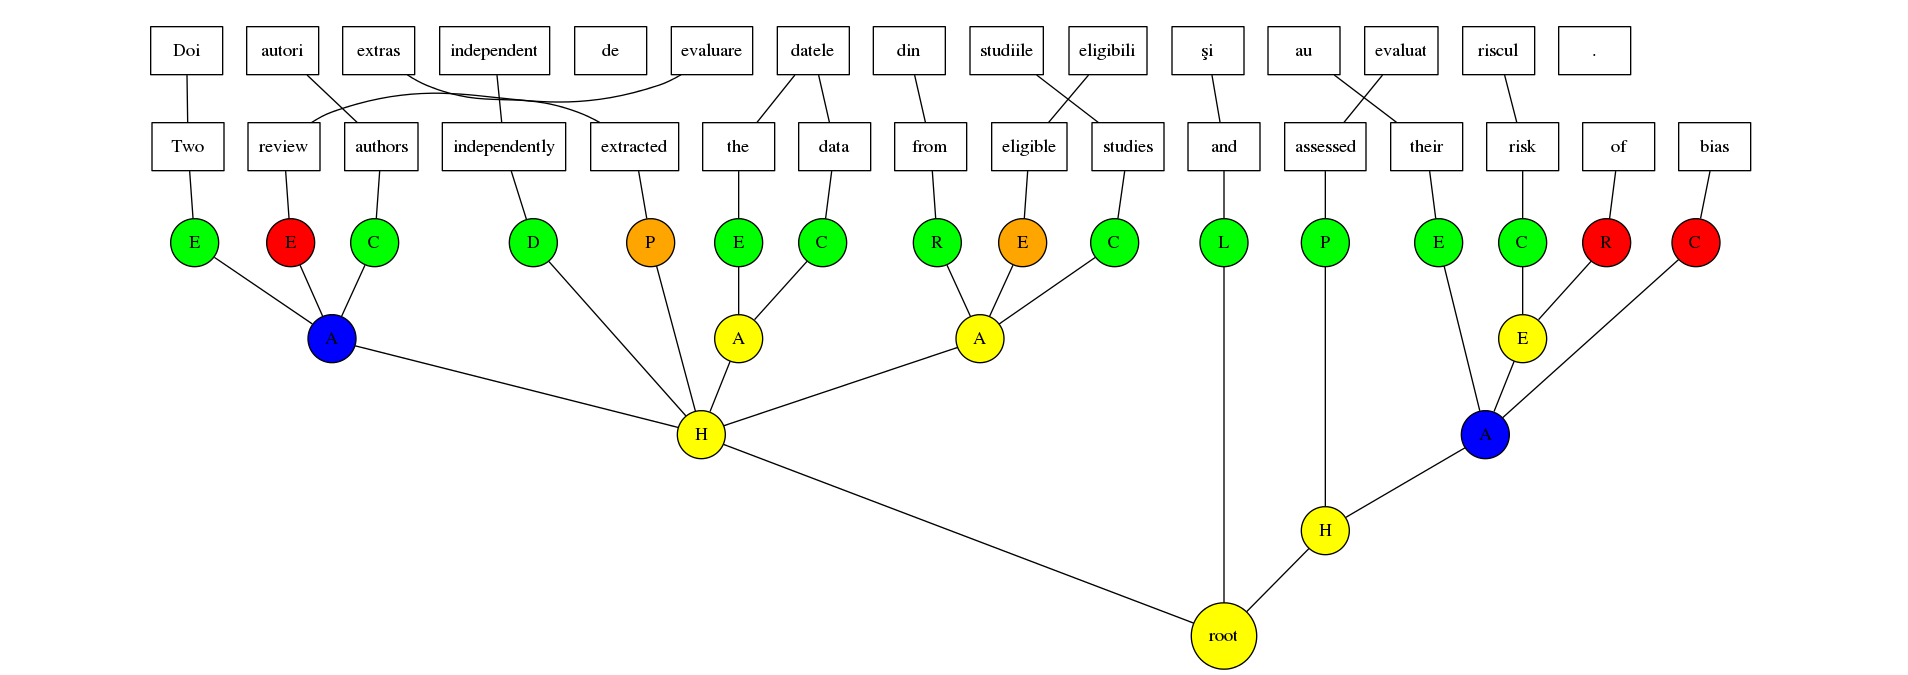
\includegraphics[width=1.1\textwidth]{tree_convert.png}
    \caption{UCCA tree on the source labelled with the MT Eval labels and aligned to the target translation. The 
    ``Acceptable'' structural nodes are yellow, the ``Bad'' ones are blue.}
    \label{fig:ucca-tree-evaluated}
\end{figure*}

%\lexi{TODO: Any chance of an example with bad structural nodes ? }
In order to visualise the UCCA evaluation results and see how the node scores are calculated, we provide an  example from the experiment. 
Looking at Figure~\ref{fig:ucca-tree-evaluated}, we can see the machine translation at the top. Below this are the word alignments to the English source. 
Each of the English words (except punctuation) are linked to UCCA lexical nodes which have been evaluated as either
correct (green), partially correct (orange) or incorrect (red). The letters inside the circles correspond to the UCCA node types
which will be important in future versions of the score. Structural nodes are either acceptable (yellow) or bad (blue). 
So for this sentence given that we have 11 green nodes, 2 orange nodes, 6 yellow nodes and in total there are 24 nodes:

\begin{displaymath}
node score = \frac{ 11  + 0.5 ( 2 ) + 6  } { 24  } * 100\\
                    = 75
\end{displaymath}

\subsection{Discussion}

In this evaluation we have proposed an evaluation which has a number of advantages:
\begin{itemize}
\item  It shows moderate IAA agreement which means that our metric is relatively reliable. It is not directly comparable to other metrics because HMEANT papers do not report IAA and they had to rely on agreement statistics which can be misleading. 
\item  We can reuse the UCCA structures on the source multiple times, and as this is the most time consuming part
of the evaluation, this makes best use of expensive expert annotators. 
\item Translation annotators do not have to try to create semantic structures on erroneous machine translation output, in fact
they do not need to create any semantic structures at all as this can be done previously by experts.
\item Errors are isolated at the point where they occur due to the separation of structure and lexical content and there
is little ambiguity about whether an error in a leaf needs to be counted multiple times as we go up the tree. 
\item UCCA provides a minimal yet complete semantic framework which is based on universal cognitive concepts. 
The structure does not rely on syntactic heads and the semantic graph is grounded directly to the words in the sentence. 
\end{itemize}

The evaluation also brought up a number of issues that will need to be resolved by either better  training or
by improving the tool. Many of these issues were reported by the annotators:
\begin{itemize}
\item Isolating errors to the point where they occur is difficult to do for humans as there is a tendency to
penalise the parent nodes for errors which occur in their children. 
\item Initially some annotators struggled to understand the distinction between lexical and structural nodes. 
\item They also had some difficulty evaluating the 
%sentence 
sentences
without their context. 
\item The annotators were unsure about how to judge incorrect morphology or tense. 
\item  The alignments were meant only as a guide and some words are unaligned or doubly aligned and this
caused some confusion. 
\item Extraneous additions on the target might not be penalised unless they fall inside the source
semantic structure.
\end{itemize}

Even though there have been a number of issues which have arisen, the UCCA evaluation has shown to be a reliable and
efficient
method for evaluating the accuracy of HimL translation systems. 
We will continue to analyse the results from this experiment and we will run an improved version of
 this evaluation in year two
of the project. 

%Comments from Juliane (Cochrane DE)
%- There weren't many, but a few mistakes in the source, that made it difficult to annotate.
%- Sometimes it was difficult to judge without context, but not very often - at least if you're familiar with the content.  
%- There were cases where the way the sentences were segmented made it difficult to annoate them in a useful way.
%- Many wrong declinations and conjugations.
%- German genus requires pronouns or articles to be repeated in lists of nouns in order to be correct, e.g. your strength and balance = Ihre Stärke und Ihr Gleichgewicht
%- There were a few out of domain vocabulary instance, e.g. "balance" being translated in the context of banking rather than the body, but only in one or two sentences, not in all where it occured. Similarly, the word "trial" got translated as "process", "study", and in the context of a court trial. 
%- A number of Cochrane or medical research specific terms was not well translated.
%- Abbreviations never got translated correctly.
%- Participle constructions often mess up the translation completely.
%- Some verbs kept getting translated as nouns or the other way round, e.g. in review author = the author of a review, review was always interpreted as a verb; falls (noun) was mostly translated as verb. 
%- Overall: both Cochrane and NHS sentences were more often bad than understandable. Only very few were acceptable for publication on our websites in my view. I guess that was expected :)
%What I mentioned earlier:
%- The past and future tense were often ignored, which is usally not a problem for future, but for past it is
%- Fairly often verbs were not translated at all (e.g. "cause" was never translated).  
%- If the verb is present, it is often in the wrong order with the subject, as it doesn't necessarily follow the same order as in English.
%- You is sometimes translated formally and sometimes informally, even in the same sentence.
%- Need a counter to know how many sentences completed
%
%Comments from Rodica (NHS Ro):
%One of the most recurrent confusions I had during my work was in connection with the word order in the MT.
%EG.  English: This review provides limited evidence that interventions...
%         Romanian: Acest studiu intervenții care furnizează dovezi limitate
%                               (This review interventions provide limited evidence)
%My question would have been how to mark the wrong or random word order in the MT translation, when the individual words appeared, so they couldn't be marked as red. 
%In most of the examples this occurred in the Romanian translations  because the default word order in Romanian is  noun + descriptive adjective(s), rather than the other way round and so, in the MT the descriptive adjectives would be first and sometimes other words would be added before the noun, which would make the sentence incomprehensible in Romanian.
%I think I mentioned to you the other questions during the work. The one that I should have asked earlier  was how far up the structure I should  mark a missing child. I understood it only once I spoke to you, but that was quite late.
%
%
%Comments from Iwona (NHS Polish)
%- Need a counter to know how many sentences completed
%1. Phrases split in wrong places, e.g. ‘depending on’, ‘there is’
%2. Certain phrases should be treated as one unit, e.g. ‘make sure’, so a leaf node for 
%marking as green, orange or red.
%3. Different sentence structure in English and Polish, e.g.
%‘our appetites often decrease’
%Machine translation: ‘our appetites often a fall’
%Correct translation:  ‘Often decreases for us appetite’
%Please note in the example above the meaning can be worked out and for that 
%reason I marked the structural node as A. However, this is bad Polish. There were a 
%number of sentences like this one, the translation of some of them made more sense 
%than others, on the whole it was difficult to annotate them. 
%4. The following is a common occurrence:
%‘before starting a new exercise programme’
%‘before’ – ‘przed rozpoczęciem’ (should be ‘przed’)
%‘starting’ – ‘przed rozpoczęciem’ (should be ‘rozpoczęciem’)
%Both leaf nodes have the same translation, but the translation appears only once in 
%the structural node. I marked the parent node as A, and the two leaf nodes as red. 
%5. Double negation in Polish causes problems at the structural level.


\subsection{Automatic Semantic Evaluation}

The results that we have gathered in this evaluation will be used as gold data to evaluate the performance of a number of automatic
metrics, to determine which of the existing metrics are most suited to evaluating accuracy.  We have also  initiated
work on developing an automatic version of the UCCA human evaluation task. For this we need an UCCA semantic parser
and data to train it, as the UCCA treebank is relatively small. We are looking at extracting further training examples from
the Prague treebank t-layer. This will be described in Deliverable D5.3, due at the end of July 2016. 

\end{document}
